\begin{algorithm}[t]
    \caption{\textsc{SkillGraph}: Skill-Augmented RL for Agents via Evolving Skill Graphs}
    \label{alg:skillgraph}
    \small
    \begin{algorithmic}[1]
    \REQUIRE Base policy $\pi_{\text{base}}$, teacher model $\mathcal{M}$, environment $\mathrm{Env}$, unlocking threshold $\theta_{\text{unlock}}$
    \ENSURE Trained policy $\pi_{\theta^*}$, evolved skill graph $\mathcal{G}^*$
    \STATE \textbf{--- Graph Construction ---}
    \STATE $\mathcal{T}^+, \mathcal{T}^- \leftarrow \text{Rollout}(\pi_{\text{base}}, \mathrm{Env})$
    \STATE $\mathcal{V} \leftarrow \mathcal{M}(\mathcal{T}^+, \mathcal{T}^-)$ \hfill $\triangleright$ Distill general \& task-specific skills
    \STATE $\mathcal{G}=(\mathcal{V},\mathcal{E}) \leftarrow \text{InitGraph}(\mathcal{V})$ \hfill $\triangleright$ Add prereq, enhance, co-occur edges
    \STATE Compute topological levels $\ell(v)$ for all $v \in \mathcal{V}$
    \STATE \textbf{--- Cold-Start SFT ---}
    \STATE $\theta \leftarrow \text{SFT}(\pi_{\text{base}},\, \mathcal{M}(\mathrm{Env}, \mathcal{G}))$; \quad $\pi_{\text{ref}} \leftarrow \pi_\theta$
    \STATE $\mathcal{V}_{\text{active}} \leftarrow \{v : \ell(v) = 0\}$; \quad $L \leftarrow 0$ \hfill $\triangleright$ Unlock level-0 skills
    \STATE \textbf{--- Closed-Loop RL Training ---}
    \FOR{epoch $= 1$ to $N$}
        \FOR{each task $d$ with type $t(d)$}
            \STATE \textbf{Graph-Aware Retrieval:}
            \STATE \quad $\mathcal{R}_{\text{seed}} \leftarrow \{v \in \mathcal{V}_{\text{active}} : \mathrm{category}(v)=\texttt{general} \vee \mathrm{category}(v)=t(d)\}$
            \STATE \quad $\mathcal{R}_{\text{BFS}} \leftarrow \text{BackwardBFS}(\mathcal{R}_{\text{seed}}, \mathcal{G}, D)$; \quad $\mathcal{R}_{\text{beam}} \leftarrow \text{ForwardBeam}(\mathcal{R}_{\text{seed}}, \mathcal{G}, B)$
            \STATE \quad $\mathcal{R}_{\text{ret}} \leftarrow \text{TopoSort}_{\mathcal{G}}(\mathcal{R}_{\text{seed}} \cup \mathcal{R}_{\text{BFS}} \cup \mathcal{R}_{\text{beam}})$ \hfill $\triangleright$ Cap at $K_{\max}$ skills
            \STATE Sample $G$ rollouts $\{\tau^{(i)}\}_{i=1}^G \sim \pi_\theta(\cdot \mid d, \mathcal{R}_{\text{ret}})$; \quad Update $\theta$ via GRPO
        \ENDFOR
        \IF{validation step}
            \STATE \textbf{Graph Evolution:}
            \STATE \textit{Node-level:} Insert / Merge / Split / Deprecate skills via $\mathcal{M}$
            \STATE \textit{Edge-level:} Reinforce paths in $\tau^+$; Discover new co-occur edges; Decay \& prune weak edges
            \STATE Recompute topological levels $\ell(v)$
            \STATE \textbf{Progressive Unlocking:} \textbf{if} $\bar{p}(L) \geq \theta_{\text{unlock}}$ \textbf{then} $\mathcal{V}_{\text{active}} \leftarrow \mathcal{V}_{\text{active}} \cup \{v : \ell(v) = L{+}1\}$; $L \leftarrow L{+}1$
        \ENDIF
    \ENDFOR
    \RETURN $\pi_\theta, \mathcal{G}$
    \end{algorithmic}
    \end{algorithm}
\vspace{10pt}
\section{Experiments}
\label{sec:experiments}
\subsection{Experimental Setup}


\begin{table}[t]
    \caption{Main results on ALFWorld and WebShop. ALFWorld reports per-subtask and overall success rates~(\%); WebShop reports task score and success rate~(\%). \textbf{Bold} and \underline{underline} denote the best and second-best results, respectively.}
    \label{tab:main}
    \centering
    \small
    \setlength{\tabcolsep}{4pt}
    \begin{tabular}{lrrrrrrr|rr}
    \toprule
    \multirow{2}{*}{Method} & \multicolumn{7}{c|}{ALFWorld} & \multicolumn{2}{c}{WebShop} \\
     & Pick & Look & Clean & Heat & Cool & Pick2 & All & Score & Succ. \\
    \midrule
    \multicolumn{10}{l}{\textit{Closed-source LLMs}} \\
    GPT-4o          & 75.3 & 60.8 & 31.2 & 56.7 & 21.6 & 49.8 & 48.0 & 31.8 & 23.7 \\
    Gemini-2.5-Pro  & 92.8 & 63.3 & 62.1 & 69.0 & 26.6 & 58.7 & 60.3 & 42.5 & 35.9 \\
    \midrule
    \multicolumn{10}{l}{\textit{Prompt-based Agentic or Memory-based Methods}} \\
    ReAct     & 48.5 & 35.4 & 34.3 & 13.2 & 18.2 & 17.6 & 31.2 & 46.2 & 19.5 \\
    Reflexion  & 62.0 & 41.6 & 44.9 & 30.9 & 36.3 & 23.8 & 42.7 & 58.1 & 28.8 \\
    Mem0            & 54.0 & 55.0 & 26.9 & 36.4 & 20.8 & 7.69 & 33.6 & 23.9 & 2.00 \\
    MemP            & 54.3 & 38.5 & 48.1 & 56.2 & 32.0 & 16.7 & 41.4 & 25.3 & 6.40 \\
    ExpeL           & 21.0 & 67.0 & 55.0 & 52.0 & 11.0 & 6.00 & 46.3 & 30.9 & 11.2 \\
    SimpleMem       & 64.5 & 33.3 & 20.0 & 12.5 & 33.3 & 3.84 & 29.7 & 33.2 & 8.59 \\
    \midrule
    \multicolumn{10}{l}{\textit{RL-based Methods}} \\
    RLOO       & 87.6 & \underline{78.2} & 87.3 & 81.3 & 71.9 & 48.9 & 75.5 & 80.3 & 65.7 \\
    GRPO       & 90.8 & 66.1 & 89.3 & 74.7 & 72.5 & 64.7 & 77.6 & 79.3 & 66.1 \\
    \midrule
    \multicolumn{10}{l}{\textit{Memory-Augmented RL-based Methods}} \\
    MemRL           & 62.8 & 38.5 & 22.2 & 12.5 &  8.00 &  0.00 & 21.4 & 29.5 &  9.20 \\
    EvolveR         & 64.9 & 33.3 & 46.4 & 13.3 & 33.3 & 33.3 & 43.8 & 42.5 & 17.6 \\
    Mem0+GRPO       & 78.1 & 54.8 & 56.1 & 31.0 & 65.0 & 26.9 & 54.7 & 58.1 & 37.5 \\
    SimpleMem+GRPO  & 89.5 & 63.6 & 60.0 & 50.0 & 64.9 & 26.3 & 62.5 & 67.8 & 46.9 \\
    SkillRL         & \underline{97.9} & 71.4 & \underline{90.0} & \underline{90.0} & \textbf{95.5} & \textbf{87.5} & \underline{89.9} & \underline{85.2} & \underline{72.7} \\
    \midrule
    \textsc{SkillGraph} (Ours) & \textbf{100.0} & \textbf{80.0} & \textbf{100.0} & \textbf{100.0} & \underline{80.0} & \underline{83.3} & \textbf{90.6} & \textbf{91.5} & \textbf{84.4} \\
    \bottomrule
    \end{tabular}
    \end{table}
    
\paragraph{Environments.}
ALFWorld~\citep{shridhar2020alfworld} is a text-based household interaction environment that covers six task categories (Pick, Look, Clean, Heat, Cool, Pick2), each requiring multi-step goal-directed manipulation. WebShop~\citep{yao2022webshop} presents a web navigation challenge in which agents must search, browse, and purchase products meeting specific user requirements. For search-augmented question answering, we evaluate on three single-hop benchmarks---NQ~\citep{kwiatkowski2019nq}, TriviaQA~\citep{joshi2017triviaqa}, and PopQA~\citep{mallen2023popqa}---and four multi-hop benchmarks---HotpotQA~\citep{yang2018hotpotqa}, 2Wiki~\citep{ho2020twowiki}, MuSiQue~\citep{trivedi2022musique}, and Bamboogle~\citep{press2023bamboogle}.

\paragraph{Baselines.}
We compare \textsc{SkillGraph} against four groups of methods. \textbf{(1) Closed-source LLMs}: GPT-4o~\citep{openai2024gpt4o} and Gemini-2.5-Pro~\citep{comanici2025gemini}, serving as strong references. \textbf{(2) Prompt-based and memory-augmented methods}: ReAct~\citep{yao2022react}, Reflexion~\citep{shinn2023reflexion}, Mem0~\citep{chhikara2025mem0}, MemP~\citep{fang2025memp}, ExpeL~\citep{zhao2024expel}, and SimpleMem~\citep{liu2025simplemem}, which use in-context experience without parameter updates. \textbf{(3) RL-based methods}: RLOO~\citep{ahmadian2024rloo} and GRPO~\citep{shao2024deepseekmath}. \textbf{(4) Memory-augmented RL methods}: MemRL~\citep{zhang2026memrl}, EvolveR~\citep{wu2025evolver}, Mem0+GRPO, SimpleMem+GRPO, and SkillRL~\citep{xia2025skillrl}. For search-augmented QA, we additionally compare against CoT~\citep{wei2022chain}, RAG~\citep{arslan2024survey}, Search-o1~\citep{li2025searcho1}, Search-R1~\citep{jin2025searchr1} and ZeroSearch~\citep{sun2025zerosearch}.

\paragraph{Implementation details.}
We adopt Qwen2.5-7B-Instruct~\citep{bai2023qwen} as the base policy $\pi_{\text{base}}$, initialized via cold-start SFT, and OpenAI o3~\citep{openai2025o3} as the teacher model $\mathcal{M}$ for skill distillation, SFT data generation, and graph evolution operations. RL training uses GRPO with learning rate $1 \times 10^{-6}$, KL coefficient $\beta=0.01$, clipping parameter $\epsilon_c=0.2$, train batch size $16$, and group size $G=8$. For graph-aware retrieval, we cap the retrieved skill sequence at $K_{\max}=8$, set backward-BFS depth $D=2$, and forward beam width $B=3$. For graph evolution, edges are initialized with weights $w=0.3$ (co-occur) and $w=0.2$ (enhance); at each validation checkpoint, successful paths receive additive reinforcement $\alpha=0.05$, all weights decay by factor $\gamma=0.99$, and edges below $w_{\min}=0.05$ are pruned. Node-level evolution uses merge threshold $\tau_{\text{merge}}=0.85$, and at most $m=3$ newly inserted skills per update. Progressive unlocking activates level-$(L{+}1)$ skills when the average success rate of level-$L$ skills exceeds $\theta_{\text{unlock}}=0.6$.

\subsection{Main Results}

\paragraph{Comparison with baselines.}
Table~\ref{tab:main} reports results on ALFWorld and WebShop. \textsc{SkillGraph} achieves the best overall performance on both benchmarks.
\textit{(i)} Notably, \textsc{SkillGraph} with a 7B open-source model substantially outperforms closed-source LLMs: it surpasses GPT-4o by $42.6$ points and Gemini-2.5-Pro by $30.3$ points on ALFWorld, and exceeds both by over $48$ points on WebShop, demonstrating that structured skill reasoning can compensate for the scale gap.
\textit{(ii)} Compared with prompt-based and memory methods, \textsc{SkillGraph} outperforms the best method (ExpeL) by $44.3$ points on ALFWorld, with the largest gains on Clean ($100.0$ vs.\ $55.0$) and Heat ($100.0$ vs.\ $56.2$). These subtasks require executing prerequisite actions in a strict order, which flat retrieval cannot enforce but graph-aware retrieval handles naturally.
\textit{(iii)} Over the vanilla GRPO baseline with the same optimizer, \textsc{SkillGraph} improves by $13.0$ and $18.3$ points on ALFWorld and WebShop respectively, directly quantifying the benefit of graph-structured skill guidance in reducing exploration burden.
\textit{(iv)} Against the strongest prior method SkillRL, \textsc{SkillGraph} achieves slightly higher ALFWorld performance while gaining $11.7$ points on WebShop. The gap stems from the evolving graph structure: graph evolution continuously refines the skill set and discovers inter-skill relations (e.g., query refinement $\to$ attribute matching $\to$ price comparison), providing higher-quality compositional guidance than a static flat skill bank.

\paragraph{Generalization to search-augmented QA.}

\begin{table}[t]
    \caption{Results on search-augmented QA. \textsc{SkillGraph} is trained on NQ$^\heartsuit$ and HotpotQA$^\heartsuit$ (in-domain) and evaluated zero-shot on the remaining five benchmarks$^\spadesuit$ (out-of-domain).}
    \label{tab:qa}
    \centering
    \footnotesize
    \setlength{\tabcolsep}{3pt}
    \begin{tabular}{lrrr|rrrr|r}
    \toprule
    \multirow{2}{*}{Method} & \multicolumn{3}{c|}{Single-Hop QA} & \multicolumn{4}{c|}{Multi-Hop QA} & \multirow{2}{*}{Avg.} \\
     & NQ$^\heartsuit$ & TriviaQA$^\spadesuit$ & PopQA$^\spadesuit$ & HotpotQA$^\heartsuit$ & 2Wiki$^\spadesuit$ & MuSiQue$^\spadesuit$ & Bamboogle$^\spadesuit$ & \\
    \midrule
    Qwen2.5-7B-Instruct  & 11.6 & 35.6 &  1.20 & 16.4 & 22.2 &  4.80 & 14.4 & 15.2 \\
    CoT   & 12.8 & 35.6 &  3.80 & 16.2 & 22.6 &  6.60 & 24.0 & 17.4 \\
    RAG      & 27.4 & 58.2 & 17.8  & 25.8 & 23.2 &  9.40 & 16.8 & 25.5 \\
    Search-o1 & 19.4 & 40.6 & 11.4  & 17.0 & 27.0 &  8.60 & 30.4 & 22.1 \\
    Search-R1         & 39.3 & 61.0 & 39.7  & 37.0 & 40.1 & 14.6  & 36.8 & 38.5 \\
    ZeroSearch        & 43.6 & 61.8 & \textbf{51.5}  & 34.6 & 35.2 & 18.4  & 27.8 & 39.1 \\
    EvolveR           & 43.5 & \underline{63.4} & 44.6  & 38.2 & \underline{42.0} & 15.6  & 54.4 & 43.1 \\
    SkillRL           & \underline{45.9} & 63.3 & 45.9  & \underline{43.2} & 40.3 & \textbf{20.2}  & \textbf{73.8} & \underline{47.1} \\
    \midrule
    \textsc{SkillGraph} (Ours) & \textbf{48.0} & \textbf{63.8} & \underline{48.5} & \textbf{44.7} & \textbf{43.4} & \underline{19.5} & \underline{72.6} & \textbf{48.9} \\
    \bottomrule
    \end{tabular}
    \end{table}
Table~\ref{tab:qa} reports results on seven QA benchmarks. Trained only on NQ and HotpotQA, \textsc{SkillGraph} achieves the highest average performance ($48.9$) and generalizes zero-shot to five unseen datasets.
On single-hop tasks, \textsc{SkillGraph} surpasses all baselines on NQ ($52.9$) and PopQA ($52.6$), improving over SkillRL by $2.1$ and $2.6$ respectively. This advantage stems from graph evolution, which keeps the skill set aligned with the evolving policy rather than relying on a fixed skill library.
On multi-hop tasks, \textsc{SkillGraph} leads on HotpotQA ($44.7$) and 2Wiki ($43.4$), where prerequisite-ordered retrieval helps decompose chained queries into sub-questions.
These results confirm that the structured skill representation learned from two training domains transfers effectively to unseen tasks, demonstrating strong generalization without task-specific adaptation.

\begin{figure}[t]
    \centering
    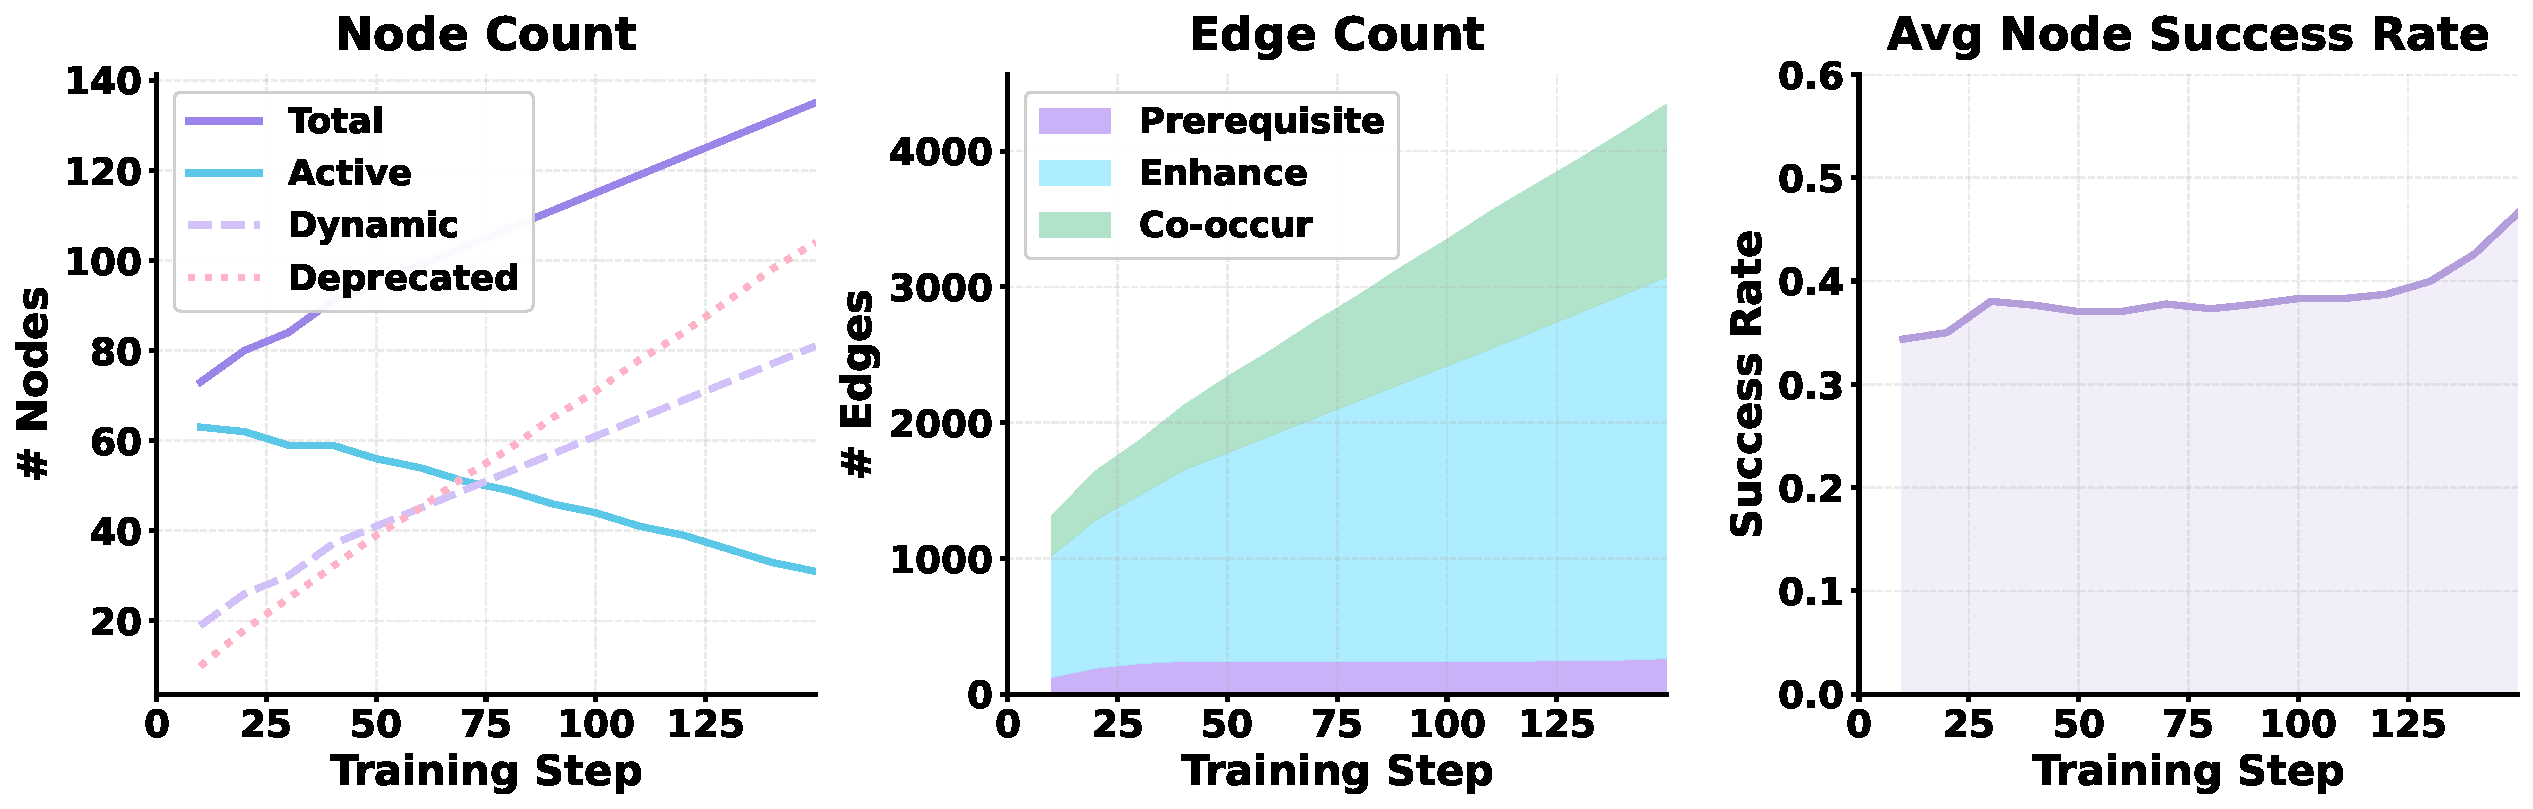
\includegraphics[width=\linewidth]{figure/skill_graph_evolution.pdf}
    \vspace{-20pt}
    \caption{Skill graph evolution over training on WebShop. Left: node counts (total, active, inserted, deprecated). Middle: edge counts by type. Right: average node success rate.}
    \label{fig:graph_evolution}
    \vspace{-10pt}
\end{figure}
\subsection{Analysis}

\begin{wraptable}{l}{0.5\textwidth}
    \vspace{-30pt}
    \caption{Ablation study on ALFWorld and WebShop success rate(\%).}
    \label{tab:ablation}
    \centering
    \small
    \begin{tabular}{lrr}
    \toprule
    Method & ALFWorld & WebShop \\
    \midrule
    \textsc{SkillGraph} & \textbf{90.6} & \textbf{84.4} \\
    \midrule
    w/o Graph Structure  & 89.9 & 72.7 \\
    w/o Graph-aware Ret. &  59.4    &  79.7  \\
    w/o Graph Evolution &  78.2  &  70.3 \\
    w/o Cold-Start SFT   &  73.4  &  67.2  \\
    \bottomrule
    \end{tabular}
    \vspace{-20pt}
\end{wraptable}
\paragraph{Ablation study.}
Table~\ref{tab:ablation} isolates each component's contribution. The components exhibit complementary strengths across environments.
On ALFWorld, removing graph-aware retrieval causes the largest single drop ($-31.2$), confirming that the rigid multi-step subtasks (e.g., Clean, Heat) critically depend on prerequisite-ordered skill sequences, consistent with the large gains reported in the main results.
On WebShop, graph evolution ($-14.1$) and graph structure ($-11.7$) contribute the most, indicating that WebShop benefits primarily from maintaining a high-quality, evolving skill set---the correct skills matter more than their ordering in this flexible navigation setting, which explains why the graph structure gap over SkillRL ($+11.7$) is larger than the retrieval ordering gap.
Cold-start SFT yields the largest combined drop ($-17.2$ on both), confirming that a good initialization is essential for RL convergence in complex agent environments.

\paragraph{Skill graph evolution dynamics.}
Figure~\ref{fig:graph_evolution} tracks graph statistics over training. Node count grows from ${\sim}20$ to ${\sim}140$ via failure-driven insertion, but the active count plateaus earlier as deprecation prunes failing skills---a self-regulating loop that prevents unbounded growth. Co-occur edges grow fastest through automatic discovery, while prerequisite and enhance edges increase steadily via path reinforcement, showing that the graph discovers relational structure beyond initial construction. The average node success rate rises confirming that evolution progressively filters low-quality skills while reinforcing useful ones.

\begin{figure}[t]
    \centering
    \begin{minipage}[t]{0.48\linewidth}
        \centering
        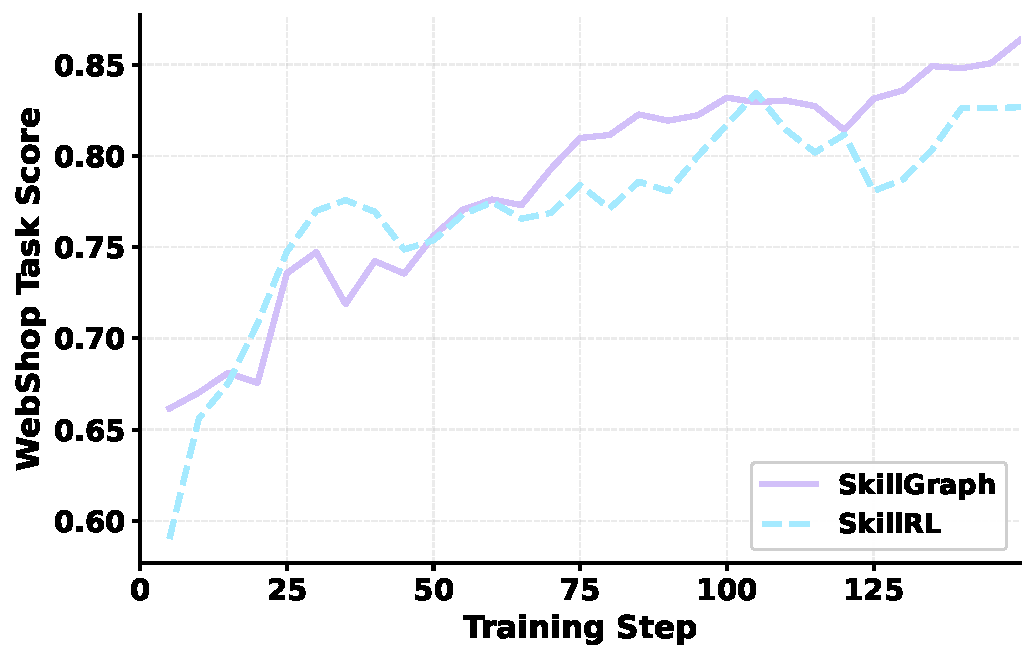
\includegraphics[width=\linewidth]{figure/webshop_task_score.pdf}
    \end{minipage}\hfill
    \begin{minipage}[t]{0.48\linewidth}
        \centering
        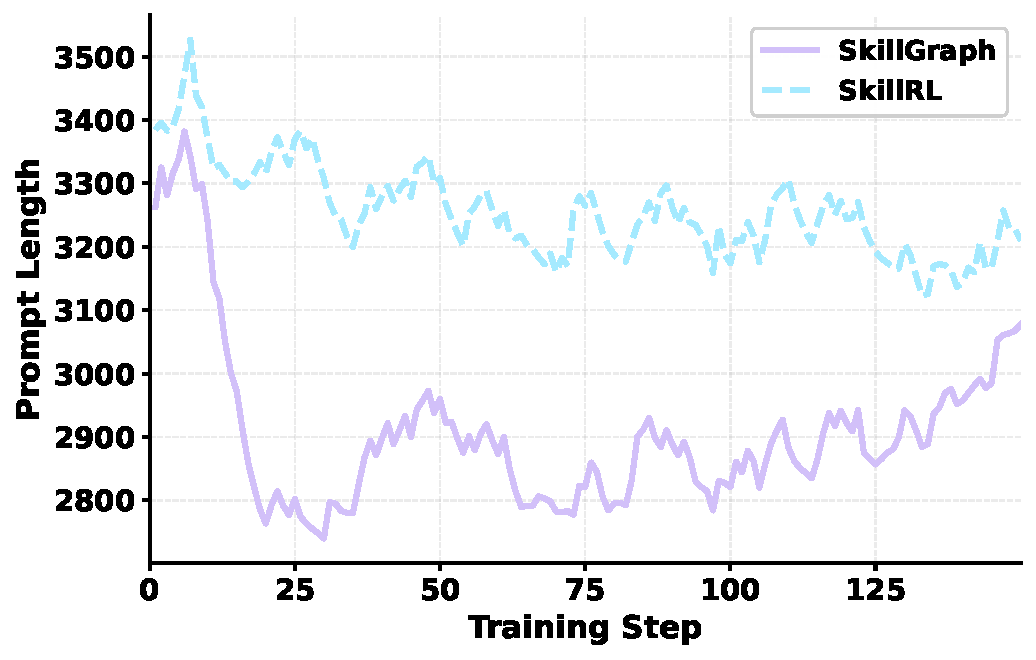
\includegraphics[width=\linewidth]{figure/prompt_length.pdf}
    \end{minipage}
    \caption{Training dynamics and context efficiency. Left: WebShop task score over training epochs. Right: average prompt length during training.}
    \label{fig:analysis_curves}
\end{figure}

\paragraph{Convergence and context efficiency.}
Figure~\ref{fig:analysis_curves}~(left) shows that \textsc{SkillGraph} surpasses SkillRL after roughly $50$ training steps and maintains a consistently higher score thereafter, converging to a superior final performance. The faster convergence is driven by dependency-ordered retrieval reducing early-stage exploration and progressive unlocking acting as an automatic curriculum. Figure~\ref{fig:analysis_curves}~(right) shows that graph-guided retrieval maintains shorter prompts than flat retrieval throughout training, because graph traversal limits the retrieved set to topologically relevant skills rather than all semantically similar entries, improving both inference cost and signal-to-noise ratio.
